\documentclass[12pt,a4paper]{article}
\usepackage[utf8]{inputenc}
\usepackage[italian]{babel}
\usepackage{amsmath}
\usepackage{amsfonts}
\usepackage{amssymb}
\usepackage{blindtext}
\usepackage{scrextend}
\usepackage{graphicx}
\usepackage{geometry}
\usepackage{listings}
\usepackage{xcolor}
\usepackage{makeidx}
\usepackage{hyperref}
\hypersetup{
colorlinks=false,
linktoc=all
}

\title{Esempi utilizzo libreria}
\author{}
\date{}
\addtokomafont{labelinglabel}{\sffamily}

\lstdefinestyle{myScalastyle}{
language=Scala,
aboveskip=3mm,
belowskip=3mm,
showstringspaces=false,
columns=flexible,
basicstyle={\small\ttfamily},
numbers=none,
numberstyle=\tiny\color{gray},
keywordstyle=\color{blue},
commentstyle=\color{olive},
stringstyle=\color{violet},
frame=none,
breaklines=true,
breakatwhitespace=true,
tabsize=3,
}



\begin{document}
    \maketitle

    \tableofcontents

    \newpage

    \section{Creazione di un cluster}\label{sec:creazioneCluster}
    E' possibile creare un cluster Mesos attraverso due modalit\`a equivalenti:
    \begin{enumerate}
        \item Istanziando un oggetto di tipo \textbf{MesosClusterBuilder} e configurando gli opportuni parametri:
        \begin{labeling}{clusterName}
            \item[clusterName]
            il nome simbolico da assegnare al cluster
            \item [masters]
            la lista di nodi che svolgeranno il ruoli di 'coordinatori' del cluster
            \item [agents]
            la lista di nodi che svolgeranno il ruoli di 'esecutori' all'interno del cluster
            \item [connection]
            username e chiave ssh per connettersi ai nodi elencati sopra
        \end{labeling}
        \begin{lstlisting}[style=myScalastyle]
            import cluster.MesosClusterBuilder

            object ClusterFromBuilder extends App {
            override def main(args: Array[String]): Unit = {
            val cluster = new MesosClusterBuilder()
            .setClusterName("Mesos-Cluster")
            .setMasters(List("207.154.204.131"))
            .setAgents(List("139.59.144.165", "207.154.193.158", "207.154.193.185"))
            .setConnection("root", "private_key_openssh", "")
            .build()
            }
            }
        \end{lstlisting}

        \item Creando un file di configurazione in formato json (Figura~\ref{fig1json}) da passare come argomento al metodo \textit{MesosCluster.fromJson}:
        \begin{lstlisting}[style=myScalastyle]
            import cluster.MesosCluster

            object CusterFromJson extends App {
            override def main(args: Array[String]) = {
            val cluster = MesosCluster.fromJson("clusterConfig.json")
            }
            }
        \end{lstlisting}
        \begin{figure}[h!]
            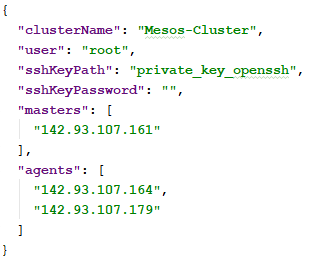
\includegraphics[scale=1]{res/esempio_json.png}
            \caption{Esempio di file di configurazione}
            \label{fig1json}
        \end{figure}

    \end{enumerate}
    In entrambi i casi \`e poi sufficiente richiamare il metodo
    \begin{lstlisting}[style=myScalastyle]
        cluster.createCluster()
    \end{lstlisting}
    per rendere operativo il cluster. Tramite questo comando, infatti, vengono installati tutti i componenti necessari(questa operazione pu\`o richiedere qualche minuto) e vengono avviati i servizi minimi per la gestione del cluster e l'esecuzione di task.



    \section{Gestione di un cluster}\label{sec:gestioneCluster}

    Una volta avviato un cluster mesos \`e possibile aggiungere e rimuovere degli agenti a seconda delle esigenze.
    Per farlo basta utilizzare i metodi \textit{addAgent} e \textit{removeAgent} di un oggetto di tipo MesosCluster

    \begin{lstlisting}[style=myScalastyle]

        import cluster.{MesosCluster, Node}

        object CusterFromJson extends App {
        override def main(args: Array[String]) = {
        val cluster = MesosCluster.fromJson("clusterConfig.json")
        cluster.createCluster()
        Thread.sleep(30000)
        //Creazione di un nuovo nodo con ip, user, ssh key ed ssh password
        val node = new Node("145.126.12.45","root","ssh_key","")
        cluster.addAgent(node)
        Thread.sleep(30000)
        cluster.removeAgent(node)
        }
        }
    \end{lstlisting}
    E' anche possibile eventualmente 'spegnere' un cluster chiamando
    \begin{lstlisting}[style=myScalastyle]
        cluster.shutdownCluster()
    \end{lstlisting}
    che ferma, in tutti i nodi, i servizi relativi al funzionamento di mesos.

    \section{Esecuzione di task all'interno del cluster}\label{sec:esecuzioneTask}
    Una volta avviato un cluster, \`e possibile eseguire dei task al suo interno.
    Gli oggetti Task possono essere creati attraverso il normale costruttore oppure un \textbf{TaskBuilder}, ed eseguiti con il comando
    \begin{lstlisting}[style=myScalastyle]
        cluster.run(task)
    \end{lstlisting}
    \begin{lstlisting}[style=myScalastyle]

        import cluster.MesosCluster
        import task.TaskBuilder

        object RunTask extends App {
        override def main(args: Array[String]) = {
        val cluster = MesosCluster.fromJson("clusterConfig.json")
        cluster.createCluster()

        //Attendiamo che il cluster sia operativo
        Thread.sleep(30000)

        val task = new TaskBuilder()
        .setId("task")
        .setMemory(1024)
        .setCpus(2)
        .setDisk(0)
        .setCmd("echo 'i'm a task' ; sleep 10")
        .build()
        cluster.run(task)
        Thread.sleep(10000)
        cluster.stop(task)
        }
        }
    \end{lstlisting}
    I parametri configurabili di un task sono:
    \begin{labeling}{instances}
        \item[id]
        id o nome del task
        \item [cpus]
        numero di cpus dedicate(default = 0.5)
        \item [memory]
        memoria RAM dedicata (default = 512)
        \item [disk]
        spazio su disco riservato (default = 0)
        \item [cmd]
        comando bash da eseguire (default = None)
        \item [container]
        container (docker o mesos) da eseguire (default = None)
        \item [env]
        mappa chiave valore di variabili d'ambiente (default = Map())
        \item [instances]
        numero di istanze del task (default = 1)
    \end{labeling}

    \section{Setup di uno stack SMACK}\label{sec:setupSmack}
    A questo punto \`e possibile , utilizzando le classi \textbf{CassandraCluster} e
    \textbf{KafkaCluster}, configurare uno stack SMACK con poche righe di codice:

    \begin{lstlisting}[style=myScalastyle]
        import cluster.MesosClusterBuilder
        import smack.SmackEnvironment

        object StartSmack extends App {
        override def main(args: Array[String]) = {

        val mesos = MesosCluster.loadFromJson("clusterConfig.json")
        mesos.createCluster()

        Thread.sleep(30000)
        val cassandra = new CassandraCluster(mesos, "cassandra-cluster")
        cassandra.start(nodes = 3, cpus = 2, memory = 2048)

        val kafka = new KafkaCluster(mesos, "kafka-cluster")
        kafka.start(brokers = 2, cpus = 2, memory = 2048)
        }
        }
    \end{lstlisting}
    Le classi deve essere instanziata con questi parametri:

    Anche in questo caso \`e possibile scalare l'architettura a seconda delle esigenze richimando i metodi
    \begin{lstlisting}[style=myScalastyle]
        cassandra.addNode(cpus,memory) e kafka.addBroker(cpus,memory)
    \end{lstlisting}
    \begin{lstlisting}[style=myScalastyle]
        object ScaleSmack extends App {
        override def main(args: Array[String]) = {
        val mesos = MesosCluster.fromJson("clusterConfig.json")
        mesos.createCluster()
        Thread.sleep(30000)
        val cassandra = new CassandraCluster(mesos, "cassandra-cluster")
        cassandra.start(nodes = 3, cpus = 2, memory = 2048)
        val kafka = new KafkaCluster(mesos, "kafka-cluster")
        kafka.start(brokers = 2, cpus = 2, memory = 2048)

        Thread.sleep(30000)
        cassandra.addNode(2, 2048)
        kafka.addBroker(1,2048)
        }
        }
    \end{lstlisting}

    \newpage
    \newgeometry{left=2cm}
    \section{Diagramma delle classi}\label{sec:diagrammaClassi}
    %%\begin{figure}[th!]
    %%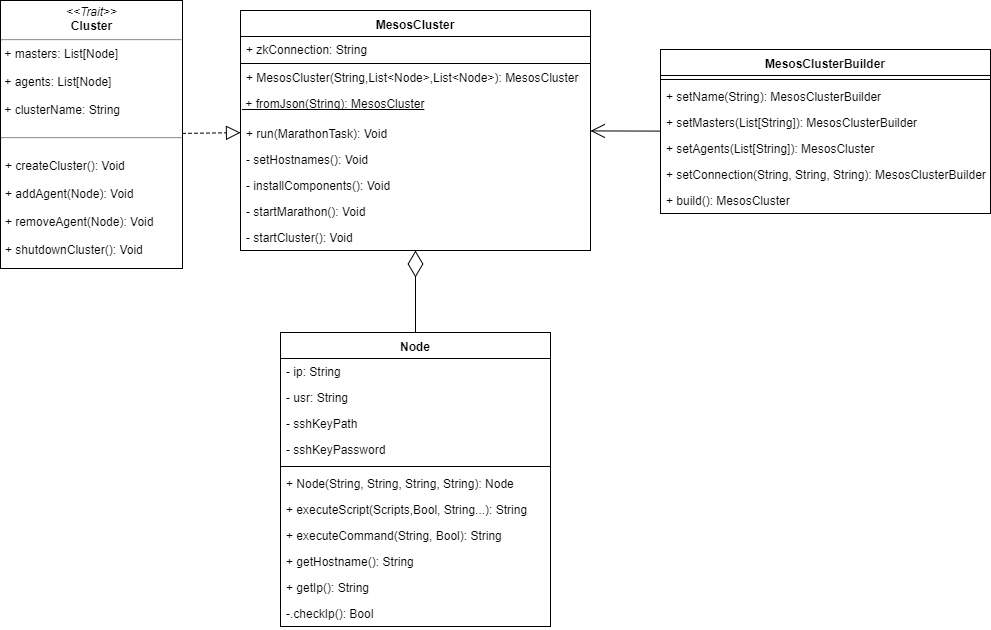
\includegraphics[scale=0.45]{res/Class_Diagram_Cluster.png}
    %%\end{figure}
    %%\begin{figure}[t!]
    %%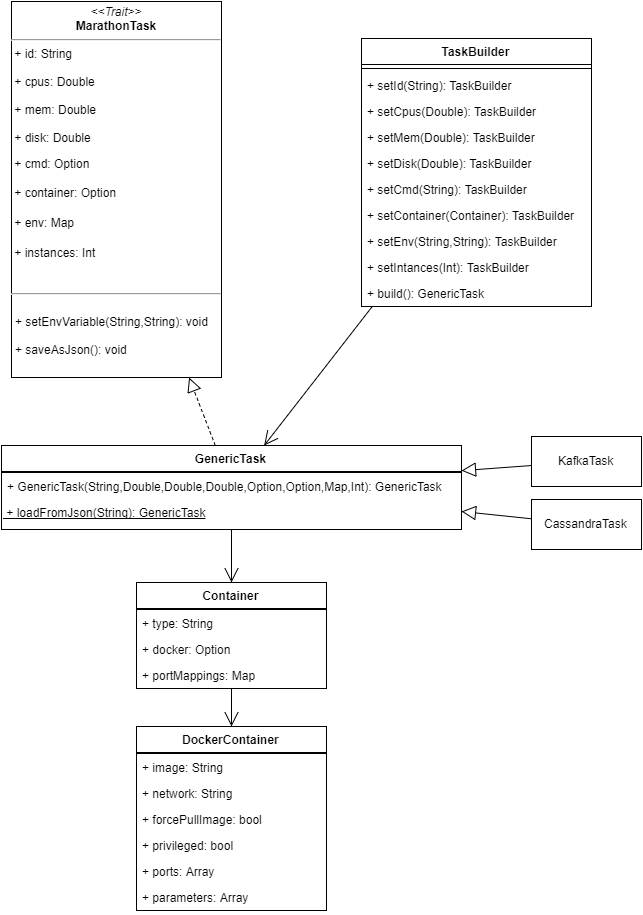
\includegraphics[scale=0.6]{res/Class_Diagram_Tasks.png}
    %%\end{figure}
    %%\begin{figure}[t!]
    %%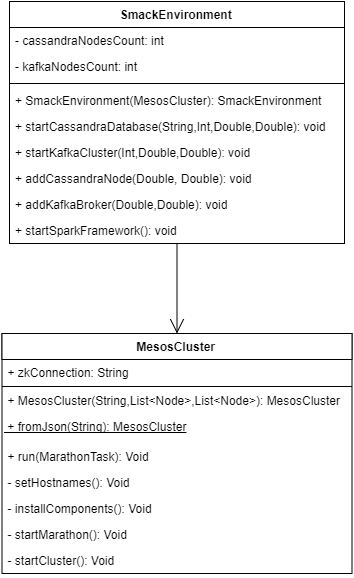
\includegraphics[scale=0.6]{res/Class_Diagram_Smack.png}
    %%\end{figure}
    \begin{figure}[!h]
        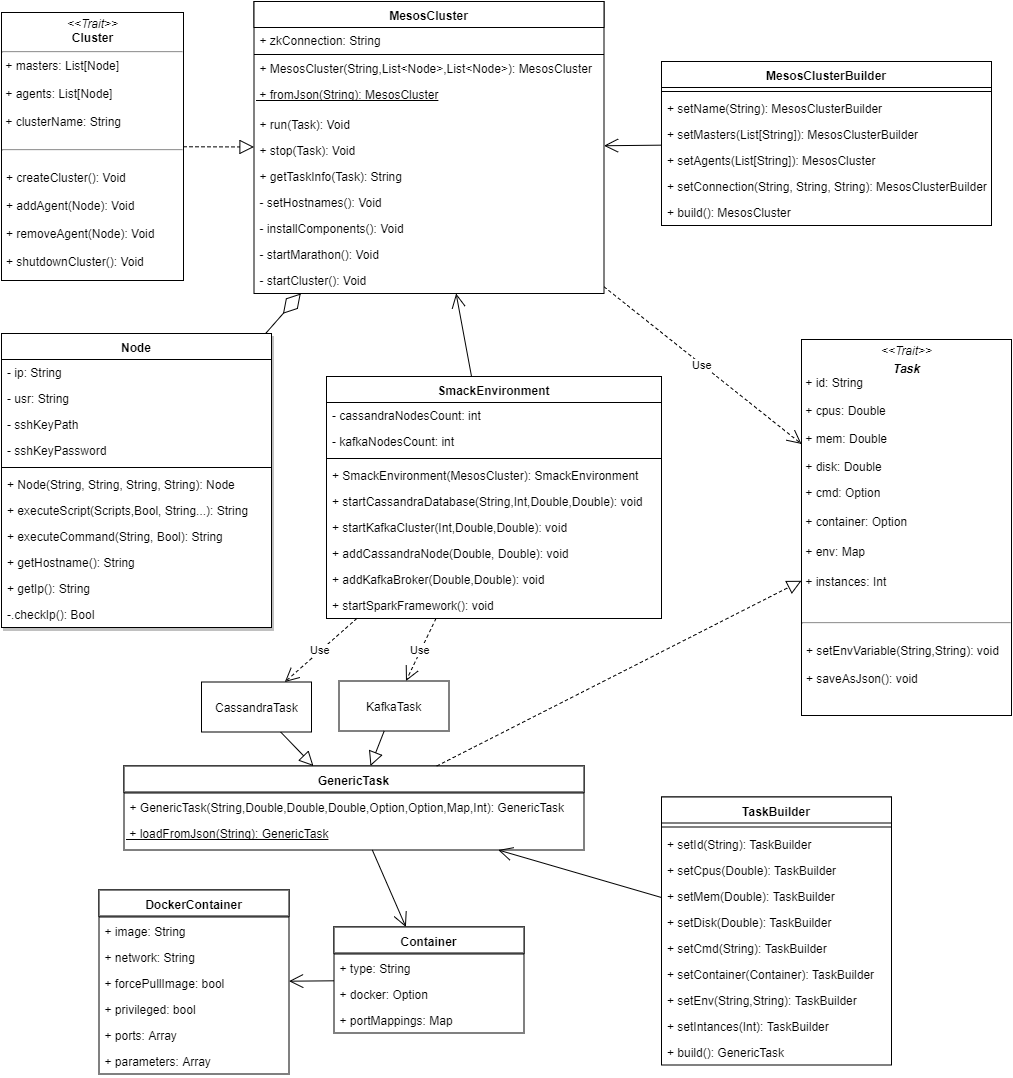
\includegraphics[scale=0.5]{res/Class_Diagram_All.png}
    \end{figure}
    \restoregeometry
\end{document}


